
\documentclass[11pt]{article}

\usepackage{graphicx} \usepackage{float} \usepackage{epstopdf}
\usepackage{xcolor}
\usepackage{amsmath}

\renewcommand{\baselinestretch}{1.2} \setlength{\topmargin}{-0.5in}
\setlength{\textwidth}{6.5in} \setlength{\oddsidemargin}{0.0in}
\setlength{\textheight}{9.1in}

\newlength{\pagewidth} \setlength{\pagewidth}{6.5in} \pagestyle{empty}

\def\pp{\par\noindent}

\newenvironment{bsmallmatrix}
  {\left[\begin{smallmatrix}}
  {\end{smallmatrix}\right]}

\begin{document}

\centerline{\bf CSE 350 -- Theory of Computation (Honors), Spring 2018}
\medskip
\centerline{Assignment 2}
\bigskip
\centerline{\bf Part B}

\newcounter{problemctr}

\addtocounter{problemctr}{1}
\addtocounter{problemctr}{1}
\addtocounter{problemctr}{1}
\bigskip
\addtocounter{problemctr}{1}
\noindent $\underline{\rm Problem\ \theproblemctr}$\pp

\noindent (A) Using the subset construction method, convert the NFA pictured here
into a DFA. Please do not include unreachable states in your construction.\\
$k=\{\{q0\},\{q1\},\{q2\},\{q3\}\},\{q0,q1\},\{q1,q3\},\{q0,q1,q3\},\{q1,q2,q3\}\}$\\
$\Sigma=\{a,b\}$\\
$s=q0$\\
$F=\{\{q3\},\{q1,q3\},\{q0,q1,q3\},\{q1,q2,q3\}\}$\\
$\delta=$\\
\begin{tabular}{|l|l|l|}
  \hline
  \textbf{Current State} & \textbf{Transition} & \textbf{New State}\\
  \hline
  \{q0\} & a & \{q1\} \\
  \hline
  \{q1\} & a & \{q3\} \\
  \hline
  & b & \{q2\} \\
  \hline
  \{q2\} & a & \{q0,q1\} \\
  \hline
  & b & \{q2\} \\
  \hline
  \{q3\} & a & \{q3\} \\
  \hline
  & b & \{q1\} \\
  \hline
  \{q0,q1\} & a & \{q1,q3\}\\ 
  \hline
  & b & \{q2\}\\
  \hline
  \{q1,q3\} & a & \{q3\}\\ 
  \hline
  & b & \{q1,q2\}\\ 
  \hline
  \{q1,q2\} & a & \{q0,q1,q3\}\\ 
  \hline
  & b & \{q2\}\\ 
  \hline
  \{q0,q1,q3\} & a & \{q1,q2,q3\}\\ 
  \hline
  & b & \{q2\}\\ 
  \hline
  \{q1,q2,q3\} & a & \{q0,q1,q3\}\\ 
  \hline
  & b & \{q1,q2\}\\ 
  \hline
\end{tabular}

\noindent (B) By placing regular expressions on the transition arrows, convert
the NFA into a regex.

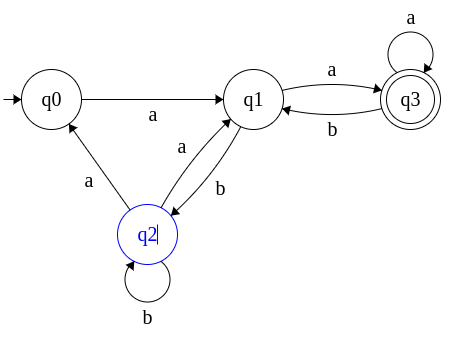
\includegraphics[scale=0.5]{4a.png}\\
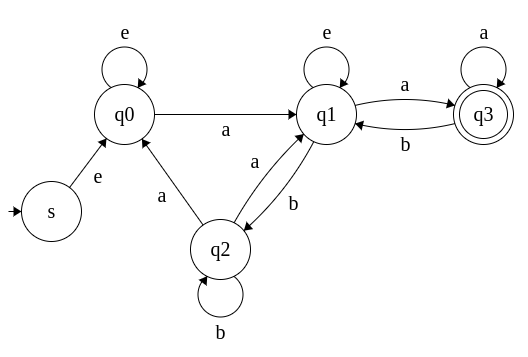
\includegraphics[scale=0.5]{4b.png}\\
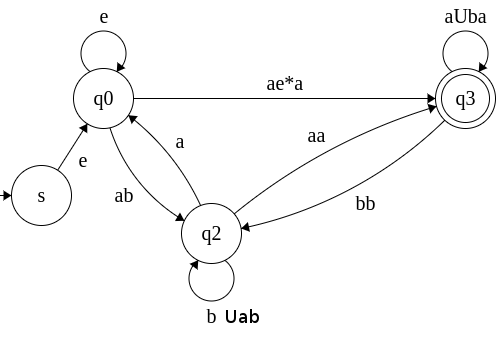
\includegraphics[scale=0.5]{4c.png}\\
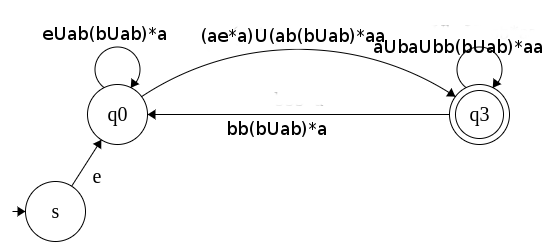
\includegraphics[scale=0.5]{4d.png}\\
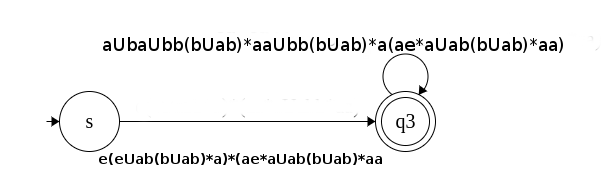
\includegraphics[scale=0.5]{4e.png}\\
The regex for the NFA is ultimately \\$e(e\cup ab(b \cup ab)^*a)^*(ae^*a\cup ab(b \cup ab)^*aa)(a\cup ba\cup bb(b\cup ab)^*aa\cup bb(b\cup ab)^*a(ae^*\cup ab(b\cup ab)^*aa))^*$\\
which can be simplified to \\$(ab(b\cup ab)^*a)^*(aa\cup ab(b\cup ab)^*aa)(a\cup ba\cup bb(b\cup ab)^*aa\cup bb(b\cup ab)^*a(a\cup ab(b\cup ab)^*aa))^*$\\
which can be simplified to \\$(ab(b\cup ab)^*a)^*(aa\cup ab(b\cup ab)^*aa)(a\cup ba\cup bb(b\cup ab)^*a(a\cup ab(b\cup ab)^*aa))^*$

\begin{figure}[H]
\hspace{-0.0in}
\centering
\end{figure}

%\bigskip
\addtocounter{problemctr}{1}
\noindent $\underline{\rm Problem\ \theproblemctr}$\pp

\noindent (A) True or False: every subset of a regular language is regular.
Justify.\\
False. All languages on an alphabet, regular or not, are a subset of the regular language $\Sigma^*$.\\
Example: In the language on the alphabet $\Sigma=\{a,b\}$, $\Sigma^*$ or $(a\cup b)^*$ is the language of all permutations of $a$ and $b$. The subset of of strings with an equal number of $a$s and $b$s is not regular.\\

\noindent (B) True or False: the union of a countable number of regular
languages is regular. Justify.\\
False. The language $a^nb^n$ for some number $n$ is uncountable. However since $n$ is a natural number, the number of elements in the language is countable, meaning it can be formed from the union of a countably infinite number of languages $a^ib^i$ where $i$ is constant.\\ 

\noindent (C) True or False: the union of two co-finite languages is regular.
Justify. (Note: a set is {\it cofinite} if its complement is finite.)\\
True. If a language is cofinite, its complement is finite, which also means that its complement is regular. Since regular languages are closed under the complement operation, that means that the lanugage is also regular.\\

\noindent (D) True or False: the intersection of a countable number of regular
languages is regular. Justify.\\
False. Regular languages are closed under the difference operation. The number of ordered pairs of natural numbers $(m,n)$ is countable (cartesian product of natural numbers with itself is countable). For the alphabet $L=\{a,b\}$, we will define a regular language, $L_{m,n}=\sigma^*-a^nb^m$ where $n$ and $m$ are constant. Since the number of languages, $L_{m,n}$, is countable, the number of languages $L_{m,n}, m\neq n$ is also countable. However, the intersection of this countable amount of regular languages is $L=a^kb^k$, or the language with an equal amount of consecutive $a$s and $b$s, which we have proven with the pumping lemma to be not regular. 

\bigskip
\addtocounter{problemctr}{1}
\noindent $\underline{\rm Problem\ \theproblemctr}$\pp
Let $x$ and $y$ be strings and $L$ a regular language. We say that $x$ and $y$
are \textbf{distinguishable} if there exists a string $z$ such that exactly one
of $xz$ and $yx$ is a member of $L$. Note that \textbf{in}distinguishability is
an equivalence relation. Define the \textbf{index of} $L$ to be the maximum
possible number of strings that are \textit{pairwise} distinguishable by $L$.

\bigskip
\noindent (A) Prove that if there exists a DFA for $L$ having $k$ states, the
index of $L$ is at most $k$.\\

Let us assume for sake of contradiction that the index of $L$ is greater than $k$ for a DFA with $k$ states.\\
This means there are greater than $k$ pairwise distinguishable strings by $L$. Since there exists a DFA with $k$ states. The minimal DFA for $L$ has at most $k$ states, meaning it has at most $k$ equivalence classes by the Myhill-Nerode theorem. Then by the pigeonhole principle, there exists at least one pair of strings $x,y$ that are distinguishable, but share the same equivalence class.\\
This forms a contradiction since this means $x$ and $y$ are also indistinguishable.\\

\noindent (B) Prove that if the index of L is $k$, there is a DFA with $k$ states that recognizes L.\\
If the index of $L$ is $k$, then there exists at most $k$ pairwise distinguishable strings by $L$. Since distinguishability means nonequivalence, there would be at most $k$ equivalence classes in $L$. (The equivalence relationship is the negation of distinguishability means that  $\forall x,y: xz,yz\in L\rightarrow$ x and y are equivalent.)\\
This means that the minimal DFA has $k$ states by the Myhill-Nerode theorem.

\bigskip
\addtocounter{problemctr}{1}
\noindent $\underline{\rm Problem\ \theproblemctr}$\pp
Let $L = \{ a^p\, |\, \mbox{ $p$ is prime} \}$. Prove that $L$ is irregular.
(\textit{Hint:} use the pumping lemma.)\\
Proof\\
Let us assume for sake of contradiction that the language $L = \{ a^p\, |\, \mbox{ $p$ is prime} \}$ is regular.\\
The language consists of strings only containing $a$s. That means that by the weak pumping lemma there exists some substring consisting only of $a$s that repeats, $a^w(a^x)^ya^z$. This means there will be some constant number of $a$s between strings in the language. This implies that the difference between any two consecutive primes is a constant. This is untrue, which can be seen in the first 3 primes: $p_1=2$,$p_2=3$,$p_3=5$.\\
This contradicts our assumption, proving that the language is not regular.

\newpage

\addtocounter{problemctr}{1}
\bigskip
\noindent
$\underline{\rm Problem\ \theproblemctr}$ (Extra Credit)\pp
\noindent

\noindent Say I have a linked list, that may or may not be corrupted. A corrupted linked
list contains a loop -- traveling along the list will eventually bring me to a
node which I have already seen.

\bigskip
\noindent (A) Determine whether the linked list is corrupted in linear time
and constant space. You cannot modify the list.

\bigskip
\noindent (B) If the list is corrupt, find the beginning of the loop in
linear time and constant space.

\end{document}
